\documentclass[11pt]{article}
\usepackage{fancyhdr}
\pagestyle{fancy}
\newcommand\course{MATH 423}
\newcommand\hwnumber{2}
\newcommand\duedate{October 13, 2019}

\lhead{Oliver Tonnesen\\V00885732}
\chead{\textbf{\Large Project \hwnumber}}
\rhead{\course\\\duedate}


\usepackage{cite}
\usepackage{url}


\usepackage{tikz}


\usepackage{float}
\usepackage{subcaption}


\usepackage{amsmath,amsfonts,amsthm}


\begin{document}
\section{Matchings}
\subsection{Matchings in graphs}

A matching in a graph is a set of edges such that any two share no vertex.
If every vertex in the graph is the endpoint of an edge in the matching, then the matching is called \textbf{perfect}.
If the graph is bipartite, and if for every vertex in the graph, we are given an ordering of preferences for each element in the other partite set, then a \textbf{stable matching} is a perfect matching where there do not exist elements $x$ and $y$, one from each partite set, such that $x$ prefers $y$ over the element to which it is already matched, and $y$ also prefers $x$ over the element to which it is already matched.



\subsection{Stable matchings}

The Stable Matching Problem (commonly called the Stable Marriage Problem, as it is often stated in terms of men and women selecting partners to marry) originated in part when David Gale and Lloyd Shapley wondered if they could design a self-enforcing job application process \cite{Kleinberg}.
That is, given a list of job candidates with an ordering of their preferred places of work, and a list of job openings with an ordering of their most suitable applicants, can one assign applicants to jobs in such a way that no job candidate would rather work somewhere that would also rather employ them? This question eventually lead to the Gale-Shapley algorithm.


\subsection{Applications}

Some potential applications of the Stable Matching Problem are load balancing clients to low-latency servers, and servers to clients that cost the least to serve \cite{LoadBalance}, assigning graduating medical students to hospitals, or helping transplant patients whose loved ones' organs are incompatible find suitable donors \cite{Kidney}.


\subsection{Examples}

Given two sets: $\{1,2,3\}$ and $\{A,B,C\}$ and the following preference lists:
\begin{align*}
	1: C,A,B&\qquad A: 1,2,3\\
	2: B,A,C&\qquad B: 3,2,1\\
	3: C,B,A&\qquad C: 1,3,2,
\end{align*}
a stable matching is:
\begin{figure}[H]
\centering
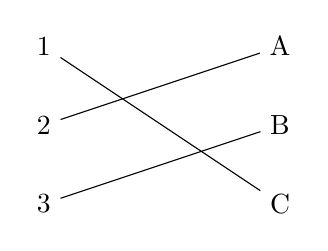
\begin{tikzpicture}[black/.style={circle,draw,fill=black,inner sep=0pt, minimum width=4pt}]
\node at (1,2) (1) {1};
\node at (1,1) (2) {2};
\node at (1,0) (3) {3};
\node at (4,2) (A) {A};
\node at (4,1) (B) {B};
\node at (4,0) (C) {C};
\draw (1) -- (C);
\draw (2) -- (A);
\draw (3) -- (B);
\end{tikzpicture}

\end{figure}


\section{Finding a stable matching}

\subsection{Gale-Shapley algorithm}

For convenience, We explain the Gale-Shapley algorithm in terms of men and women marrying.
The algorithm works by allowing women to change their mind, instead of being forced to marry the first man who proposes to her despite a more optimal partner proposing later on.
The algorithm operates as follows:

\noindent
Repeat the following until all men and women are engaged:\\ (1) Find an unpaired man $m$.
\ (2) Have $m$ propose to the woman $w$ highest on his preference list and to whom he has not already proposed.
\ (3) If $w$ prefers $m$ to her current partner (if any) then $w$ dumps her current partner, and $m$ and $w$ become engaged.


\subsection{Examples}

Given two sets: $\{m1,m2,m3,m4,m5\}$ and $\{w1,w2,w3,w4,w5\}$ and the following preference lists:
\begin{align*}
	m1: w3,w2,w5,w1,w4&\qquad w1: m3,m5,m2,m1,m4\\
	m2: w1,w2,w5,w3,w4&\qquad w2: m5,m2,m1,m4,m3\\
	m3: w4,w3,w2,w1,w5&\qquad w3: m4,m3,m5,m1,m2\\
	m4: w1,w3,w4,w2,w5&\qquad w4: m1,m2,m3,m4,m5\\
	m5: w1,w2,w4,w5,w3&\qquad w5: m2,m3,m4,m1,m5
\end{align*}

We apply the Gale-Shapley algorithm.
Between any two figures below we add as many edges as we can until we reach a conflict.
In such a conflicting scenario, a dashed line represents the new proposed partnership, green indicates that the current partnership remains, and red indicates that the standing partnership is broken in favour of the new one.

\begin{figure}[H]
\centering
\begin{subfigure}{.33\textwidth}
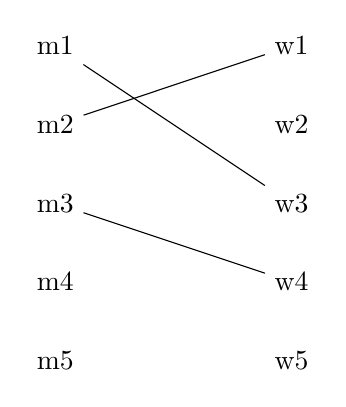
\begin{tikzpicture}[black/.style={circle,draw,fill=black,inner sep=0pt, minimum width=4pt}]
\node at (1,4) (m1) {m1};
\node at (1,3) (m2) {m2};
\node at (1,2) (m3) {m3};
\node at (1,1) (m4) {m4};
\node at (1,0) (m5) {m5};
\node at (4,4) (w1) {w1};
\node at (4,3) (w2) {w2};
\node at (4,2) (w3) {w3};
\node at (4,1) (w4) {w4};
\node at (4,0) (w5) {w5};

\draw (m1) -- (w3);
\draw (m2) -- (w1);
\draw (m3) -- (w4);
\end{tikzpicture}

\end{subfigure}
\begin{subfigure}{.33\textwidth}
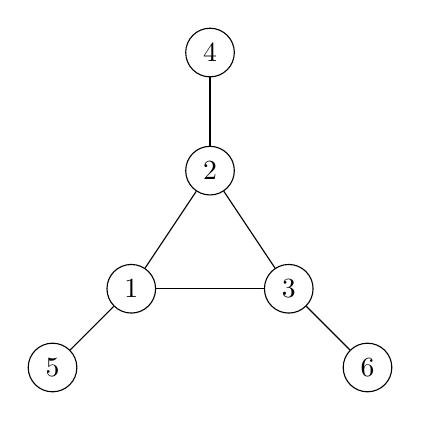
\begin{tikzpicture}[black/.style={circle,draw,fill=black,inner sep=0pt, minimum width=4pt}]
\node[circle,draw] at (1,1) (1) {1};
\node[circle,draw] at (0,0) (5) {5};
\node[circle,draw] at (3,1) (3) {3};
\node[circle,draw] at (2,2.5) (2) {2};
\node[circle,draw] at (2,4) (4) {4};
\node[circle,draw] at (4,0) (6) {6};

\draw (1) -- (2);
\draw (1) -- (3);
\draw (2) -- (3);
\draw (4) -- (2);
\draw (5) -- (1);
\draw (6) -- (3);
\end{tikzpicture}

\end{subfigure}
\end{figure}
\begin{figure}[H]
\centering
\begin{subfigure}{.33\textwidth}
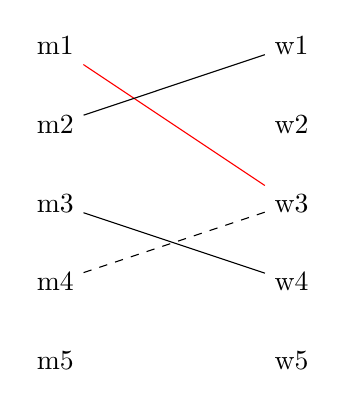
\begin{tikzpicture}[black/.style={circle,draw,fill=black,inner sep=0pt, minimum width=4pt}]
\node at (1,4) (m1) {m1};
\node at (1,3) (m2) {m2};
\node at (1,2) (m3) {m3};
\node at (1,1) (m4) {m4};
\node at (1,0) (m5) {m5};
\node at (4,4) (w1) {w1};
\node at (4,3) (w2) {w2};
\node at (4,2) (w3) {w3};
\node at (4,1) (w4) {w4};
\node at (4,0) (w5) {w5};

\draw[red] (m1) -- (w3);
\draw (m2) -- (w1);
\draw (m3) -- (w4);
\draw[dashed] (m4) -- (w3);
\end{tikzpicture}

\end{subfigure}
\begin{subfigure}{.33\textwidth}
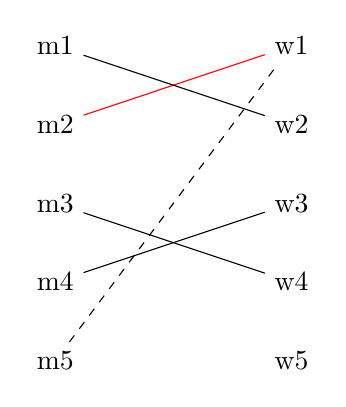
\begin{tikzpicture}[black/.style={circle,draw,fill=black,inner sep=0pt, minimum width=4pt}]
\node at (1,4) (m1) {m1};
\node at (1,3) (m2) {m2};
\node at (1,2) (m3) {m3};
\node at (1,1) (m4) {m4};
\node at (1,0) (m5) {m5};
\node at (4,4) (w1) {w1};
\node at (4,3) (w2) {w2};
\node at (4,2) (w3) {w3};
\node at (4,1) (w4) {w4};
\node at (4,0) (w5) {w5};

\draw[red] (m2) -- (w1);
\draw (m3) -- (w4);
\draw (m4) -- (w3);
\draw (m1) -- (w2);
\draw[dashed] (m5) -- (w1);
\end{tikzpicture}

\end{subfigure}
\end{figure}
\begin{figure}[H]
\centering
\begin{subfigure}{.33\textwidth}
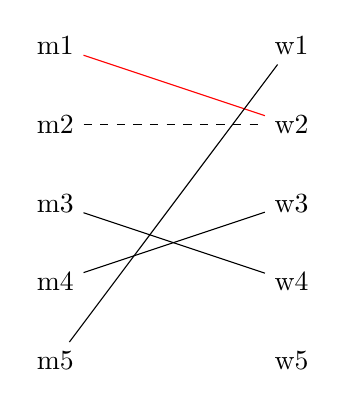
\begin{tikzpicture}[black/.style={circle,draw,fill=black,inner sep=0pt, minimum width=4pt}]
\node at (1,4) (m1) {m1};
\node at (1,3) (m2) {m2};
\node at (1,2) (m3) {m3};
\node at (1,1) (m4) {m4};
\node at (1,0) (m5) {m5};
\node at (4,4) (w1) {w1};
\node at (4,3) (w2) {w2};
\node at (4,2) (w3) {w3};
\node at (4,1) (w4) {w4};
\node at (4,0) (w5) {w5};

\draw (m3) -- (w4);
\draw (m4) -- (w3);
\draw[red] (m1) -- (w2);
\draw (m5) -- (w1);
\draw[dashed] (m2) -- (w2);
\end{tikzpicture}

\end{subfigure}
\begin{subfigure}{.33\textwidth}
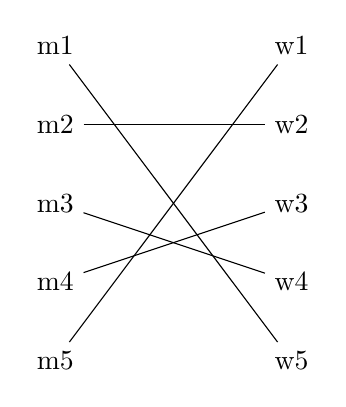
\begin{tikzpicture}[black/.style={circle,draw,fill=black,inner sep=0pt, minimum width=4pt}]
\node at (1,4) (m1) {m1};
\node at (1,3) (m2) {m2};
\node at (1,2) (m3) {m3};
\node at (1,1) (m4) {m4};
\node at (1,0) (m5) {m5};
\node at (4,4) (w1) {w1};
\node at (4,3) (w2) {w2};
\node at (4,2) (w3) {w3};
\node at (4,1) (w4) {w4};
\node at (4,0) (w5) {w5};

\draw (m3) -- (w4);
\draw (m4) -- (w3);
\draw (m5) -- (w1);
\draw (m2) -- (w2);
\draw (m1) -- (w5);
\end{tikzpicture}

\end{subfigure}
\end{figure}


\subsection{Correctness of the algorithm}

We want to show that by the end of the algorithm's execution, we're left with a stable matching.
\newline

\noindent
We first show that the algorithm produces a matching:
\newline

At any point during the execution of the algorithm, if $m$ and $w$ are matched, then $m$ was previously unmatched, and $w$ was either previously not matched, or she dumped her previous partner to be with $m$.
In either case, $m$ is matched only with $w$, and $w$ is matched only with $m$, so what we're left with is indeed a matching.
\newline

\noindent
We now show that the matching the algorithm produces is perfect:
\newline

Suppose that there exists a man $m$ who is unmatched by the end of the algorithm's execution.
Then, since there are an equal number of men and women, and since everyone is matched with at most one other person, there must exist a woman $w$ who is also unmatched.
This is not possible, since at some point, $m$ would have proposed to $w$, and $w$ would have accepted, since she was unmatched at the time.
Thus the matching produced must also be perfect.
\newline

\noindent
Finally, we show that the perfect matching produced by the algorithm is stable:
\newline

Assume that the matching the algorithm produces is not stable.
Then there exists a pair $(m,w)$ such that $m$ and $w$ are not married, but $m$ prefers $w$ over his wife, and $w$ prefers $m$ over her husband.
Let $w'$ and $m'$ be $m$'s and $w$'s spouses, respectively.
Since $w'$ is lower on $m$'s preference list than $w$, $m$ must have proposed to $w$ earlier in the algorithm's execution, but $m'$ is lower on $w$'s preference list than $m$, so $w$ would have either not accepted $m'$'s proposal, or would have dropped $m'$ in favour of $m$ at the time of $m$'s proposal.
Thus our assumption was false, and so no such pair $(m,w)$ exists, and the matching is therefore stable. \cite{Kleinberg}



\section{Further remarks}

A particularly interesting application of Gale and Shapley's algorithm, described in \cite{Kidney}, is helping transplant patients receive kidneys.
If a transplant patient has a friend or family member who is willing to give their kidney, but for some reason is incompatible with the recipient, then the Gale-Shapley algorithm can be used to find a stable matching between kidney donors and recipients such that every transplant patient receives a kidney with which they are compatible.
During the first year this program was run, it increased the rate of kidney transplants by around twenty times, and its creator, Alvin Roth, received a Nobel Prize in Economics.


% \section{References}
\bibliography{p2}
\bibliographystyle{plain}


\end{document}
